\chapter{The Central Limit Theorem}

\section{Introduction}

In this lab, we'll use Monte Calro techniques to demonstrate the
convergence of the Binomial distribution to the Poisson distribution,
and then demonstrate the Central Limit Theorem.

\section{The Poisson Limit}

The Poisson distribution follows from the Binomial distribution in the
limit that $n_{\rm try} \to \infty$.  Recall that the mean value of
the Poisson distribution is $\bar{m} = \epsilon \, n_{\rm try}$.  If
we kept the success rate $\epsilon$ as a parameter, than any finite
value of $\epsilon$ would cause the mean of the distribution to diverge to infinity.
If instead we hold the new parameter $\lambda$ constant, and set:
\begin{displaymath}
\epsilon = \frac{\lambda}{n_{\rm try}}
\end{displaymath}
we see that $\epsilon \to 0$ as $n_{\rm try} \to \infty$ and the mean
of the Poisson distribution remains at the fixed value $\lambda$.

We'll explore this limit numerically simply by taking $n_{\rm try}$ to
the large (but finite) value of 1000.  Re-run your Monte Carlo
simulation using the parameters $n_{\rm try} = 1000$, $n_{\rm exp} =
1000$, and $\epsilon = \lambda / n_{\rm try}$.  For now, take $\lambda
= 2.0$.  Instead of the Binomial distribution, compare your simulation to the Poisson distribution PDF
using the {\tt poisson.pmf} function:
\begin{verbatim}
from scipy.stats import poisson
xpred = edges[:-1]
ypred = nexp * poisson.pmf(xpred, lamb) 
\end{verbatim}
Note that the first argument of the {\tt pmf} function is the array of
positions to evaluate the function at, while the second is the Poisson
parameter $\lambda$.  Also note that sadly {\tt lambda} is a reserved word
in python, and so you cannot use it as a variable name.

\begin{figure}[htbp]
\begin{center}
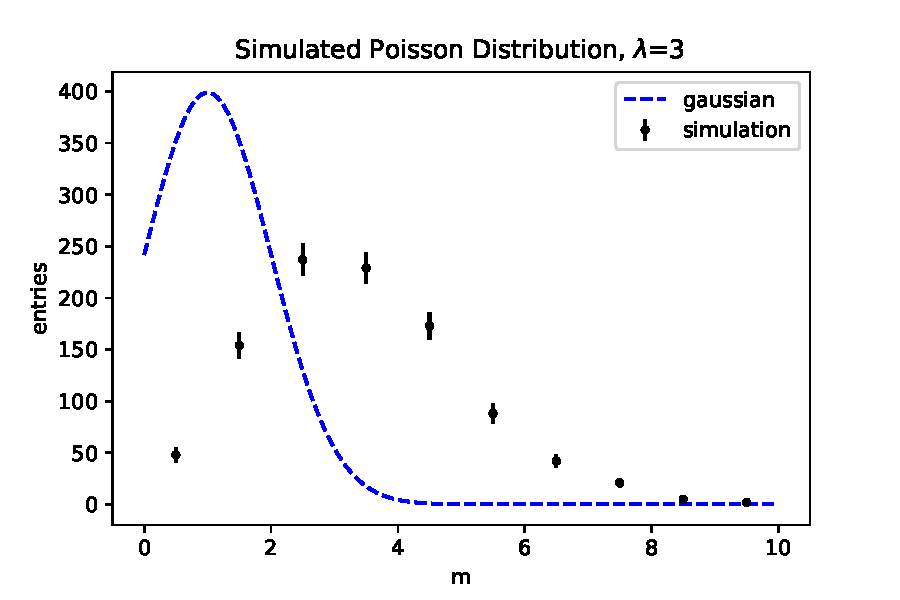
\includegraphics[height=0.22\textheight]{figs/labs/distributions/poisson.pdf}
\end{center}
\caption{\label{fig:poisson} Example of the expected result for the Monte Carlo simulation data in comparison to the Poisson PDF for for $\lambda=2$. }
\end{figure}

\begin{plot} In the Poisson limit, compare the output of your Monte Carlo simulation to the Poisson PDF
for $\lambda=5.2$.
%for two different values of $\lambda$:  2.0, 5.2.  
Plot the histogram with 15 bins for the outcomes: 0,1,2,3,...,14.  
An example for $\lambda=2$ is shown in Fig.~\ref{fig:poisson}.
\end{plot}

%Using {\tt np.mean} and {\tt np.var}, check that mean and variance of
%your distributions is as you expect in each case, and record the
%results in your log book.

This is a \textbf{sign-off point} for this lab.  Make certain you can
explain your code, and that it is as neat and organized as you can
manage.

\section{The Gaussian Limit}

\begin{figure}[htbp]
\begin{center}
\begin{tabular}{cc}
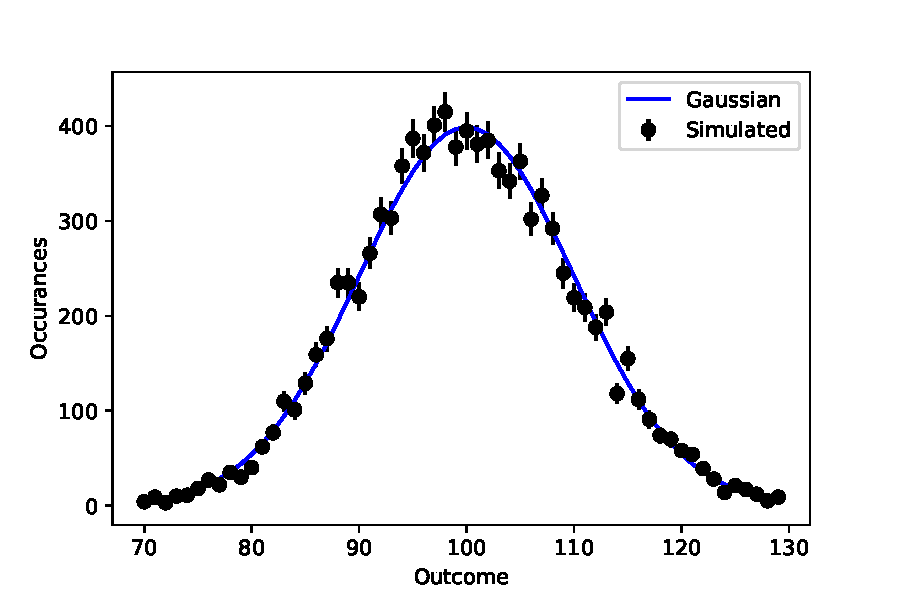
\includegraphics[height=0.22\textheight]{figs/labs/distributions/gauss_finebins.pdf} &
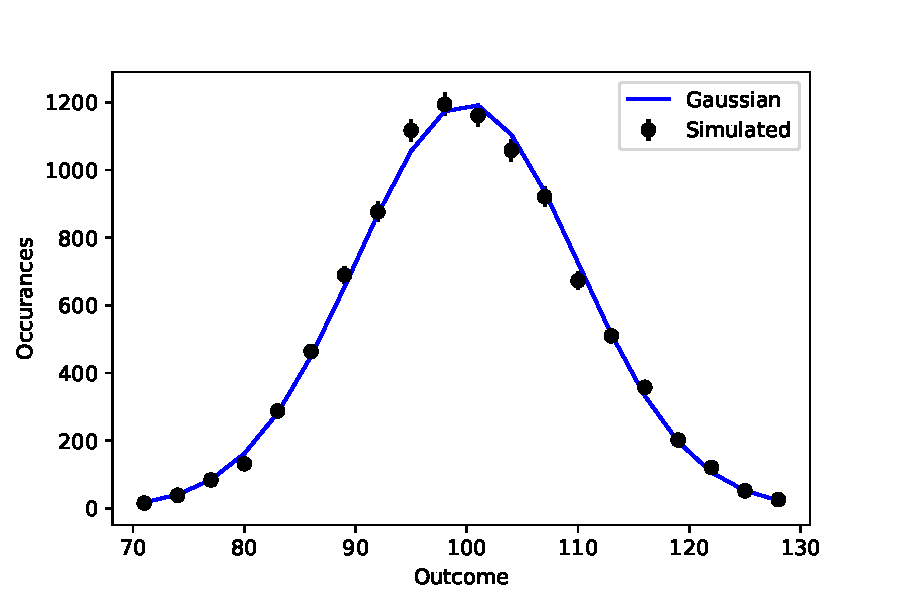
\includegraphics[height=0.22\textheight]{figs/labs/distributions/gauss.pdf} \\
(a) & (b) \\
\end{tabular}
\end{center}
\caption{\label{fig:gauss} Example of the expected result for the Monte Carlo simulation data in comparison to the Gaussian PDF for $\lambda=100$. }
\end{figure}

As the mean value $\lambda$ of the Poisson distribution gets larger,
the Poisson distribution resembles the Gaussian distribution.  We will
simulate this numerically by taking our Monte Carlo simulation in the
Poisson limit, as above, with $\lambda = 100$.  Initially use
integer bins inclusively in the range 70 to 130, e.g.:
\begin{verbatim}
counts,edges = np.histogram(m,bins=60,range=(70,130))
\end{verbatim}
and compare with the Gaussian (also called normal) distribution PDF, e.g.:
{\tt scipy.stats.norm.pdf} function:
\begin{verbatim}
from scipy.stats import norm
xpred = edges[:-1]
ypred = nexp * norm.pdf(xpred, loc=lamb, scale=lamb**0.5). 
\end{verbatim}

\begin{plot} Set the parameter {\tt loc} to the mean value, and the parameter {\tt
  scale} to $\sigma$.  Recall that in the Poisson limit $\sigma^2 =
\lambda$, which is why we set {\tt scale=lamb**0.5} in the example.
This should reproduce the plot in Fig.~\ref{fig:gauss}a. \end{plot}

You should see that 60 bins is rather unwieldy.  We'll reduce the number
of bins, but that's actually a bit more complicated than you might
expect: non-integer bins with discrete data is about the most
challenging binning you can tackle.  You'll have to do the following:
\begin{itemize}
\item While keeping the range of 70 to 130, set the number bins to {\tt bins=20} when filling your histogram.
\item Our trick to use edges[:-1] will no longer work, since now the data for each bin is associated with a range of values in the bin.  Each bin is now 3 integers wide. If we live this as is, edges[:-1] will position the x value of the bin at its leading edge: 70, 73, 76 , ......  and the data will be plotted with an observable bias.  For continuous data, we often simply use the middle of the bin:
\begin{verbatim}
cbins = (edges[:-1] + edges[1:])/2.  
\end{verbatim}
This would position the x value of the bins at 71.5, 74.5. 77.5, ..... and that seems more reasonable choice. 
In this specific case of discrete data which doesn't extend  all the way to the right edge this is still slightly biased. The first bin in our example represents the count of all outcomes in the range from 70 (inclusive) to below 73 (exclusive). So its center should be at 71.  To be precise for this specific case, the x position we should use for plotting the contents of each bin is:
\begin{verbatim}
cbins = (edges[:-1] + edges[1:] -1 )/2 
\end{verbatim}
\item The normalization of the PDF to the data now requires an additional scale factor to account for the wider bins (which integrate more probability).  You need to scale by an additional factor of 3 to account for the fact that each bin is 3 integers wide.
\end{itemize}

\begin{plot} Using the techniques described above, reproduce Fig~\ref{fig:gauss}b, which shows that the Binomial distributions becomes a Gaussian distribution as the mean value of the distribution becomes large. \end{plot}

\begin{figure}[htbp]
\begin{center}
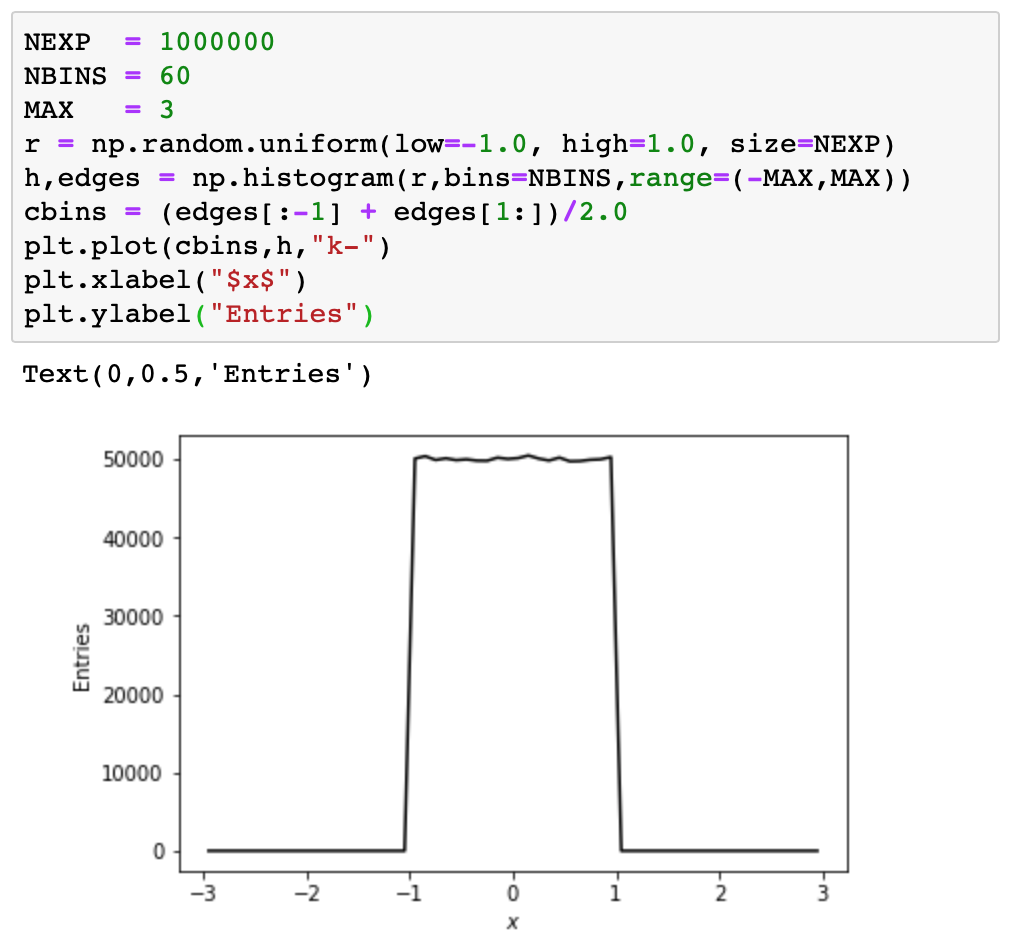
\includegraphics[width=0.75\textwidth]{figs/labs/uncertainties/step.png}\\
\end{center}
\caption{\label{fig:samplingstep} Sampling from the uniform distribution. }
\end{figure}

\begin{figure}[htbp]
\begin{center}
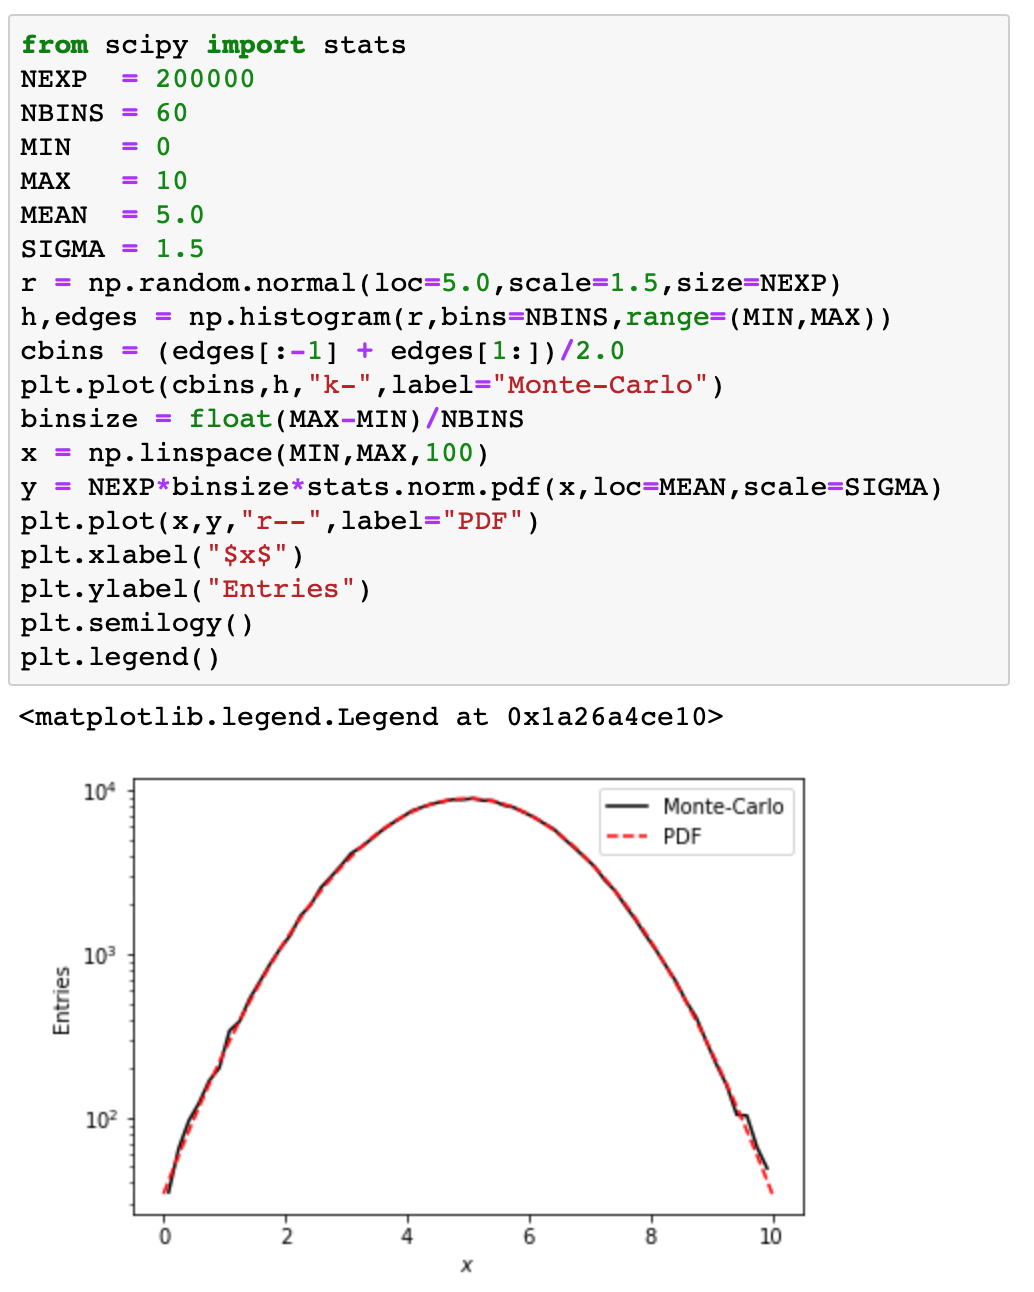
\includegraphics[width=0.75\textwidth]{figs/labs/uncertainties/gaussian.png}\\ 
\end{center}
\caption{\label{fig:samplinggauss} Sampling from the Gaussian distribution and comparison with the Gaussian PDF.}
\end{figure}

Scientific python provides functions to draw random samples according
to various distributions.  In today's lab, we will draw samples
uniformly in the interval $[-1,1]$, as demonstrated in Fig.~\ref{fig:samplingstep}.   The line
\begin{verbatim}
r = np.random.uniform(low=-1.0, high=1.0, size=NEXP)
\end{verbatim}
creates a NumPy array {\tt r} which contains {\tt NEXP} entries, with
each entry chosen uniformly and randomly in the range from -1 to 1.
In the example, these events are displayed in a histogram.  When
plotting histograms with plenty of statistics (one million entries
here) and fine binning (60 bins here) it is usually preferable to use
lines instead of points with error bars for plotting the histograms,
as is done in this example.  Notice, however, that even with one
million events, there are still statistical fluctuations which prevent
the curve from being perfectly smooth.

In Fig.~\ref{fig:samplinggauss}, entries are instead drawn from the Gaussian distribution with the line:
\begin{verbatim}
r = np.random.normal(loc=5.0,scale=1.5,size=NEXP).
\end{verbatim}
The histogram is plotted with a logarithmic $y$ scale:
\begin{verbatim}
plt.semilogy()
\end{verbatim}
which results in the Gaussian distribution appearing as a parabola.  The histogram is compared to the Gaussian PDF appropriately normalized:
\begin{verbatim}
x = np.linspace(MIN,MAX,100)
y = NEXP*binsize*stats.norm.pdf(x,loc=MEAN,scale=SIGMA)
\end{verbatim}


\section{Demonstration of the Central Limit Theorem}

In this section, you'll show that average value of random variables
chosen uniformly from -1 to 1 approaches a Gaussian distribution,
consistent with the central limit theorem.  First create a 2-D array
of size {\tt NEXP} by {\tt NAVG} filled with uniform random values in
the interval from -1 to 1, as follows:
\begin{verbatim}
r = np.random.uniform(low=-1.0, high=1.0, size=(NEXP,NAVG))
\end{verbatim}
Then calculate averages values from {\tt NAVG} entries:
\begin{verbatim}
x = np.sum(r, axis=1)/float(NAVG)  
\end{verbatim}
From the Central Limit Theorem, we expect the entries in x to approach a Gaussian distribution.

\begin{plot}  Set {\tt NEXP} to 1000000 for plenty of statistics.
Produce three different histograms with 40 bins covering the range
from -1.2 to 1.2 for three values {\tt NAVG}: 1,2, and 3.  Plot all
three histogram in the same graph with appropriate legend. \end{plot}

Your plot will show that already for three contributions to the average, the result looks quite Gaussian on a linear scale.  For more precise comparison, we will use a log scale and compare to the PDF.

\begin{plot} Calculate {\tt NEXP}$=1000000$ average values {\tt x} for {\tt NAVG}$=10$.  Calculate the mean value of the entries in {\tt x} using the {\tt np.mean} function.  Calculate $\sigma$ for the entries in $x$ by taking the square root of the output from the {\tt np.var} (variance) function.  Produce a histograms with 20 bins covering the range
from -0.5 to 0.5 for the average values.  Compare with a Gaussian distribution, appropriately normalized, using your calculated values from the  mean and sigma.  Plot both the histogram and PDF on the same graph, including an appropriate legend.  Use a logarithmic $y$ axis. \end{plot}

\section{Propagation of Uncertainties}

\begin{figure}[htbp]
\begin{center}
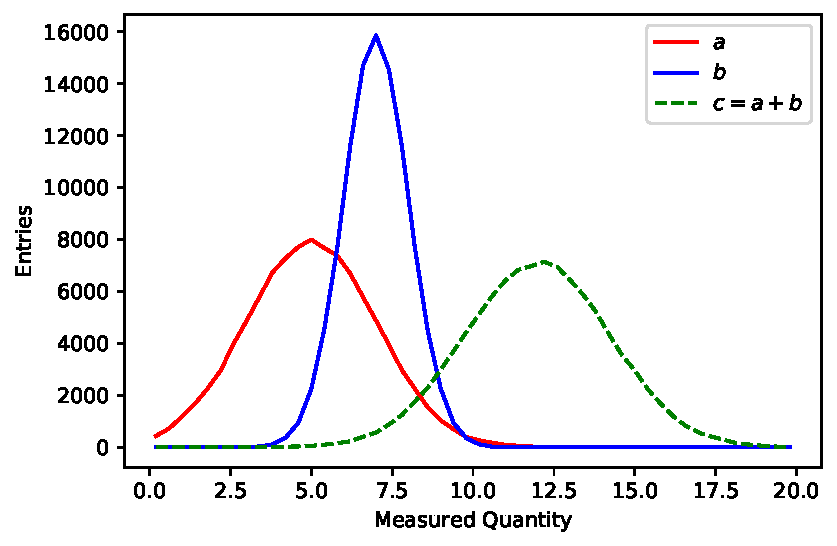
\includegraphics[width=0.75\textwidth]{figs/labs/uncertainties/addunc.pdf}\\
\end{center}
\caption{\label{fig:addunc} Simulation of many measurements of the quantity $c = a + b$. }
\end{figure}

Consider two measured values $a \pm \sigma_a$ and $b \pm \sigma_b$.  If we calculate the quantity $c = a + b$ or $c = a - b$, the uncertainty on the calculated value $c$ is given by:
\begin{displaymath}
\sigma_c = \sqrt{\sigma_a^2 + \sigma_b^2}.
\end{displaymath}
If instead, we calculate $c = a * b$ or $c = a/b$ the fractional uncertainty on $c$ is given by:
\begin{displaymath}
\frac{\sigma_c}{c} = \sqrt{\left(\frac{\sigma_a}{a}\right)^2 + \left(\frac{\sigma_b}{b}\right)^2}.
\end{displaymath}
In this section, you'll develop a numerical simulation for the
propagation of uncertainties under addition, subtraction,
multiplication, and division.  An example, for $c = a + b$ is shown in Fig.~\ref{fig:addunc}.

Pick values for $a$, $b$, $ \sigma_a$ and $ \sigma_b$ for simulating
subtraction: $c=a-b$. Record them out in your logbook. Choose values
that are different from what is plotted in Fig.~\ref{fig:addunc}.

\begin{plot} 
Simulate the measurement $a$ by drawing 100,000 random samples from a
Gaussian distribution with mean $a$ and sigma $\sigma_a$, and do
likewise for $b$.  Calculate the values $c = a -b $ from the $a$ and
$b$ values.  Plot the distribution of all three variables (as in
Fig.~\ref{fig:addunc}) as histograms with 50 bins and an appropriate
range.  Calculate the mean and variance of the simulated $c$ values
and compare to your expectations from the standard propagation of
uncertainties.
\end{plot} 

This is a \textbf{sign-off point} for this lab. 

Pick values for $a$, $b$, $\sigma_a$ and $\sigma_b$ for simulating
division: $c=a/b$. Record them in your logbook.  Choose values that
are will allow you to see the distributions of $a$, $b$, and $c$ all
on the same plot.

\begin{plot}
Simulate the measurements $a$ and $b$ using the same procedure as in the previous plots, but with your new values.  Calculate the values of $c = a/b $ from
the $a$ and $b$ values.  Plot the distribution of all three variables (as in
Fig.~\ref{fig:addunc}) as histograms with 50 bins and an appropriate
range.  Calculate the mean and variance of the simulated $c$ values
and compare to your expectations from the standard propagation of
uncertainties.
\end{plot}
























